\documentclass{article}

% NeurIPS 2026 template.
%   default (no option) = anonymized double-blind submission mode  <-- use for the workshop submission
%   [final]             = camera-ready (deanonymizes; add author block + ack below)
\usepackage{neurips_2026}
\usepackage[utf8]{inputenc}
\usepackage[T1]{fontenc}
\usepackage{hyperref}
\usepackage{url}
\usepackage{booktabs}
\usepackage{amsmath}
\usepackage{amssymb}
\usepackage{graphicx}
\usepackage{float}
\usepackage{xcolor}

% Workshop-mandated footnote (CfP: "Submitted to/Accepted at/Published in ...").
\makeatletter
\renewcommand{\@noticestring}{Submitted to the AI for Science workshop (NeurIPS 2026).}
\makeatother

\title{Verifying Agentic Scientific Workflows from Primitive Evidence with GRACE}

% Submission mode renders "Anonymous Author(s)" regardless of this block.
% CAMERA-READY: author block lives in CAMERA_READY_NOTES.txt (kept out of the submitted source).
\author{Anonymous Author(s)}
\begin{document}
\maketitle
\begin{abstract}
Agentic AI systems produce scientific results through long autonomous workflows, and the verification layers they carry are their own: self-assessments, plausibility checks, and generated reports. We show these layers can carry no signal. In the public artifact corpus of an autonomous detector-design agent, all 64 preserved physics-verification records return \texttt{plausible: true} with empty issue lists, spanning runs whose headline results include a retyped constant reported as a 204.62\% improvement, a hardcoded detection efficiency of 1.0, and a placeholder narrated as physics. We propose \emph{calibrated artifact auditing}: every claim is re-derived from the most primitive surviving evidence rather than the agent's intermediates or self-reports; a failure diagnosis is accepted only if it reproduces the claimed number to all quoted digits and survives an empirically measured false-positive rate on decoy targets; and the auditor itself is calibrated by fault injection, shipping with measured detection profiles and a characterized blind spot rather than an implicit completeness claim. A five-stage implementation audits the full eighteen-run corpus (3{,}142 numeric claims) in under an hour on a laptop, rediscovers every manually established failure mechanism from primitive evidence, corrects one of them, and---via a moment-inversion technique that reconstructs an analyzed file's summary statistics from archived error formulas---exposes two analyses that consumed stale data existing nowhere in the recorded provenance. We state the method's provenance preconditions and release the pipeline.
\end{abstract}

\section{Introduction}

Agentic systems built on large language models now execute complete scientific workflows: they read papers, write and run simulation and analysis code, interpret outputs, and report conclusions across dozens of autonomous steps \citep{grace, hellert2026, diefenbacher2025, moreno2026, chung2026}. The question of whether their outputs can be trusted is therefore no longer hypothetical, and the field's current answer is largely \emph{self}-verification: agents carry plausibility checkers, structured self-assessments, and verification sub-agents, and their demonstrations are validated by the agent's own account of its work.

This paper reports a measurement that should end confidence in that arrangement, and proposes what to do instead. In the public artifact release of GRACE, an autonomous agent for particle-detector design and simulation \citep{grace, gracedata}, the verification layer demonstrably fired: the reasoning traces of eight runs preserve 64 structured physics-verification records. Every one of them returns \texttt{plausible: true} with an empty issue list. The same corpus, audited externally, contains an order-of-magnitude geometry error that the agent's own validator rejected once and then accepted on an unmodified retry, a headline ``204.62\% improvement'' whose optimized yield is a retyped baseline scaled by a retyped percentage, a detection efficiency of 100\% corresponding to the literal assignment \texttt{baseline\_detection\_efficiency = 1.0}, and a defaulted placeholder whose statistics the generated report narrated as a physical effect. The run responsible for most of these defects reported success with all sixteen planned steps completed and \texttt{failed\_steps: 0}, after a trace containing five step errors and one regeneration. Self-assessment, in this corpus, carries \emph{no signal} separating genuine results from artifacts.

The constructive claim is that external verification of such workflows is tractable, cheap, and---critically---\emph{calibratable}. We propose \textbf{calibrated artifact auditing}, a method defined by three commitments:

\begin{enumerate}
  \item \textbf{Primitive evidence only.} Every quantitative claim is traced to, and re-derived from, the most primitive surviving record of the computation (here, per-event execution logs), never from the agent's intermediate results files, prose, or self-reports, which are treated as claims requiring evidence rather than as evidence.
  \item \textbf{Exact, null-calibrated diagnosis.} When a claim cannot be reproduced, a generating mechanism is accepted only if it reproduces the claimed number to all quoted digits \emph{and} survives an empirical false-positive measurement: the identical search rerun on jittered decoy targets of equal precision must not match at chance level.
  \item \textbf{Calibrate the auditor.} The audit itself is a measuring instrument. Known defects are injected into clones of a real run, detection is scored per stage against rules fixed before injection, and the audit ships with measured detection profiles and characterized blind spots rather than an implicit claim of completeness.
\end{enumerate}

The third commitment is, to our knowledge, new to this setting, and it is the one we most want the community to adopt. A verifier evaluated only on the defects it happened to find is in the same epistemic position as the agent it audits.

We instantiate the method as a five-stage pipeline and evaluate it on the complete eighteen-run GRACE corpus. Our contributions: (i) the method and its preconditions (\S\ref{sec:method}); (ii) a reference implementation whose expensive human steps---hypothesis formation and re-derivation---are mechanized as calibrated formula search and differential re-execution (\S\ref{sec:pipeline}); (iii) a corpus-scale evaluation accounting for 3{,}142 numeric claims, rediscovering all manually established mechanisms and finding new defect classes, including stale-input contamination exposed by a moment-inversion technique (\S\ref{sec:eval}); and (iv) a fault-injection calibration of the auditor itself, measuring a union-of-detectors coverage structure with one characterized blind spot (\S\ref{sec:calibration}).

\section{Related work}

Verification of AI-generated science is nascent. Execution-scored benchmarks evaluate generated physics code by running it \citep{phitsbench}, capability probes measure model performance on research tasks \citep{prlbench}, and recent work argues for surfacing the assumptions inside AI-generated analyses \citep{hammad2026}. Reproducibility infrastructure in experimental physics, exemplified by REANA and LHC workflow preservation \citep{reana}, answers whether a preserved result can be \emph{rerun}. The method here answers two prior questions: whether a claimed result was ever computed at all, and whether it was computed from the data the workflow actually produced. It requires artifacts an order of magnitude lighter than a preserved workflow, and it is complementary to rerun infrastructure rather than a substitute. A companion measurement addresses the orthogonal hazard of hindsight contamination in the models backing such agents.
% TODO (post-acceptance): cite the extended journal version and the contamination companion explicitly; omitted during double-blind review.

\section{The method and its preconditions}
\label{sec:method}

\paragraph{Provenance tiers.} Every quantity is assigned a tier: \textsc{log} for values derived from per-event execution records (primitive evidence); \textsc{json} for numeric leaves of results files (intermediates); \textsc{report} for numeric strings in generated prose (terminal claims). Verification flows strictly upward: a \textsc{report} claim is supported only by tracing it to \textsc{json} and then to \textsc{log}; agreement between intermediates is recorded as copying, not verification.

\paragraph{Verdicts.} Each numeric claim receives exactly one verdict: \emph{verified} (reproduced from primitive evidence by identity), \emph{copy} (verbatim inter-intermediate duplicate), \emph{diagnosed} (reproduced only by a nontrivial mechanism passing the calibration gates below), \emph{unexplained} (no mechanism in the bounded search matches---a deliberately conservative bucket), or \emph{unevaluable} (inputs absent from the archive, with the archival gap itself recorded as a finding). Coverage is reported as fractions over the full denominator, never as a list of findings.

\paragraph{Preconditions.} The method applies to corpora satisfying a minimum provenance floor: per-event (or equivalently primitive) text logs retained for every execution, and generated code retained verbatim and identifiable (e.g., by content hash). These are cheap---orders of magnitude smaller than binary data products---and we argue they are the minimum any agentic scientific system should ship. Two further requirements, motivated by defects found in the evaluation, extend the floor: content-hashing of \emph{input} files at read time against the workflow's write manifest (without which stale-input contamination is invisible), and an execution-status and output-attribution manifest (without which content-addressed script retention cannot establish which script produced which file). Appendix~\ref{app:checklist} tabulates the full standard against the failure class each item prevents.

\section{Reference implementation}
\label{sec:pipeline}

The pipeline mechanizes the two expensive steps of a manual audit---mechanism hypothesis and re-derivation---and runs five stages. On the evaluation corpus it completes in under an hour on a laptop with standard Python, no accelerators, and no access to the original computing environment.

\paragraph{Stage 1: null-calibrated mechanism search.} For each \textsc{report} claim and \textsc{json} leaf, a bounded formula grammar is searched over the run's quantity pool: identity; mean and standard deviation of any numeric family, with fallback variants appending or substituting a placeholder 1.0; ratios; energy-scaled ratios (the unit-loss class); percent differences; and percentage-scaled values $a(1+b/100)$ (the transcription-and-rescale class). The target's own leaf is removed from the pool before pair formulas run. A match must reproduce every printed digit at the claim's precision. Three guards keep the search evidential. Pair formulas are attempted only for targets with $\geq$4 significant figures; matches with multiplicity $>$5 are rejected as chance-level; and every surviving diagnosis is assigned an empirical false-positive rate by rerunning the identical search on 100 seeded, jittered decoy targets of equal precision. When mean and standard deviation of the same family variant jointly match a reported value--uncertainty pair, the diagnosis is promoted to \emph{corroborated} with a joint null measured directly on jittered value--uncertainty decoy pairs, alongside the product of the individual rates. Calibration cuts both ways: on the evaluation corpus it certified one diagnosis at a measured joint null of zero in 100 decoy pairs while eleven single-formula matches in the same run carried decoy rates of 44--99\% and stayed screening verdicts. Low-precision targets match \emph{some} grammar formula most of the time (measured decoy rates versus precision in Appendix~\ref{app:nullcal}), which is precisely why uncalibrated formula-matching is inadmissible as evidence.

\paragraph{Stage 2: dataflow analysis.} Each generated script is parsed to an abstract syntax tree and analyzed with name-level, flow-insensitive taint propagation over literal, file-derived, and external sources, with container mutations propagating taint. An output (a \texttt{RESULT:} print or \texttt{json.dump} field) reachable only from literal assignments is flagged and severity-classified by label semantics (physics class: yield, efficiency, resolution, quenching, significance; configuration class: counts, positions, geometry). The same pass detects existence-guarded silent skips, where a file-existence test dominates a \texttt{continue} on a path feeding an output.

\paragraph{Stage 3: physics-invariant battery.} Checks computable from primitive evidence alone, with no claim tracing: bounds on fraction-type quantities; a photostatistics floor $\sigma/\mu \gtrsim 1/\sqrt{\bar N_{\mathrm{PE}}}$ tested against reported resolutions with $\bar N_{\mathrm{PE}}$ from logs (binomial detection of a fixed photon count sits slightly below the Poisson value, so the test fires only below $0.8$ of the floor); a batched-run suppression test comparing log-derived response at batched versus unbatched settings; and a linearity residual scan. This is the \emph{binding} verification layer whose absence in the agent caused the failures the audit finds, demonstrated retrospectively.

\paragraph{Stage 4: differential re-execution.} The archive excludes binary event files but retains the per-event logs from which analysis inputs are reconstructible. The pipeline synthesizes the excluded event files from logs, rewrites cluster-absolute paths into a sandbox, re-executes every generated script under a 150\,s timeout, and diffs each regenerated \textsc{json} leaf against the archive. A \textsc{match} verifies the computation end-to-end mechanically; a \textsc{diverge} localizes a defect and names the value the correctly fed computation would have produced. One complementarity is essential: re-execution certifies that the archived script deterministically reproduces the archived output, while \emph{derivation from data} is a separate property---a script whose outputs are literals regenerates them identically and is caught only by Stage 2. The calibration of \S\ref{sec:calibration} measures this complementarity directly.

\paragraph{Stage 5: claim accounting.} Every numeric claim receives an identifier and a verdict; the corpus-level table is generated by one command. A table-row consistency check flags report rows in which multiple high-precision cells have no support anywhere in the archive.

\section{Evaluation on a public agentic physics corpus}
\label{sec:eval}

The evaluation corpus is the public GRACE benchmark release \citep{gracedata}: 1{,}248 files across 18 archived agentic runs (twelve reporting success, six ending in process-level failure) on a pinned LLM backbone, spanning two simulation frameworks (Opticks and Celeritas arms, in two framework versions each) and both paper-driven and prompt-driven tasks. Two of its properties match the method's preconditions: the Opticks arms log one line per simulated event (the Celeritas arms log every hundredth event), and generated scripts are retained by content hash. Its gitignore excluded all binary data products, which the method tolerates by log-synthesis (Stage 4). Three results files (\texttt{projective\_performance\_analysis.json}, \texttt{ams\_optimization\_results.json}, \texttt{bgo\_performance\_metrics.json}) are truncated mid-object and fail to parse, so their leaves enter no column of the accounting; the truncation pattern, a key with no value at the end of the file, is the signature of a serializer raising partway through a dump. A prior manual audit of the two paper-driven runs, requiring several person-days, established a set of failure mechanisms by hand; it serves as the ground-truth reference for whether the mechanized audit recovers known defects without hypotheses supplied.

\subsection{Claim accounting}

\begin{table}[t]
\centering
\caption{Corpus accounting over all 18 runs, by arm. \emph{Log-verified}: reproduced from per-event logs by identity. \emph{Copies}: verbatim inter-file duplicates. \emph{Diagnosed}: reproduced only by a nontrivial mechanism passing the Stage-1 gates (a screening category; only mechanisms confirmed by independent evidence are asserted as findings). \emph{Unexplained}: no match in the bounded grammar---a conservative bucket including low-precision values and prose restatements. \emph{HC}: physics-class script outputs reachable only from literal assignments. \emph{Skips}: existence-guarded silent omissions. Per-run rows appear in Appendix~\ref{app:perrun}.}
\label{tab:accounting}
\begin{tabular}{lrrrrrr}
\toprule
Arm (runs) & Log-ver. & Copies & Diagnosed & Unexpl. & HC & Skips \\
\midrule
Celeritas v4 (6) & 37 & 304 & 99 & 316 & 2 & 4 \\
Celeritas v7 (6) & 89 & 506 & 259 & 685 & 17 & 0 \\
Opticks v5 (3)   & 21 & 182 & 28 & 262 & 24 & 0 \\
Opticks v9 (3)   & 39 & 120 & 62 & 133 & 18 & 2 \\
\midrule
Total (18)       & 186 & 1112 & 448 & 1396 & 61 & 6 \\
\bottomrule
\end{tabular}
\end{table}

The pipeline accounts for 3{,}142 numeric claims (Table~\ref{tab:accounting}); in the mechanized accounting, targets whose inputs are absent from the archive are not tracked as a separate column and fall within the conservative unexplained bucket. Three observations matter for verification practice. First, only 186 claims (6\%) are verifiable against primitive evidence by identity, while 1{,}112 (35\%) are copies between intermediates: the corpus \emph{looks} heavily cross-confirmed while most agreement is duplication, which is exactly the structure that defeats consistency-based checking (\S\ref{sec:calibration}). Second, 61 physics-class outputs across ten runs are reachable only from literal constants, including a script that computes per-energy quenching factors in a loop, discards them, and writes a hand-transcribed literal in their place under the comment \texttt{\# Use values from previous step analysis}. We name this \emph{transcription hardcoding}: the agent's stdout-mediated memory between steps makes transcription the path of least resistance, and nothing in a results file distinguishes a transcribed constant from a computation. Third, the unexplained bucket (44\%) is reported as such: a bounded, calibrated search that cannot certify a derivation says so, rather than absorbing ambiguity into apparent coverage.

\subsection{Rediscovery of known mechanisms}
\label{sec:rediscovery}

Without hypotheses supplied, the pipeline rediscovered from primitive evidence every quantitative mechanism the manual audit had established, and replaced the manual reading of one of them with an exact-digit derivation (complete arithmetic in Appendix~\ref{app:arithmetic}): the headline ``204.62\% improvement'' as a retyped constant, with the optimized yield 4491.29 reproduced to all stored digits as the cross-energy baseline mean 1474.39 scaled by that constant (the log-reconstructed true result is a uniform $\sim$28.6\% improvement, physically sensible and sublinear in the 33.3\% coverage increase); the reported quenching mean and standard deviation (0.631, 0.264) as the statistics of two log-derived values plus a placeholder 1.0, corroborated at a measured joint decoy null of zero in 100 decoy pairs; a systematic yield suppression at exactly the energy where execution was batched, appearing in three run--particle combinations across two unrelated geometries at factors 0.47, 0.47, and 0.22; and the exact existence-check responsible for a silent input omission. The generated report had narrated the placeholder's statistics as a convergence to unity at 5\,MeV, offered as either an artifact or a physical effect; the agent's self-assessment recorded sixteen completed steps and zero failed steps. The geometry default of the introduction lives in the extraction layer, upstream of any number the five stages consume, and remains a source-inspection finding.

\subsection{Case study: stale-input contamination by moment inversion}
\label{sec:phantom}

\begin{figure}[t]
\centering
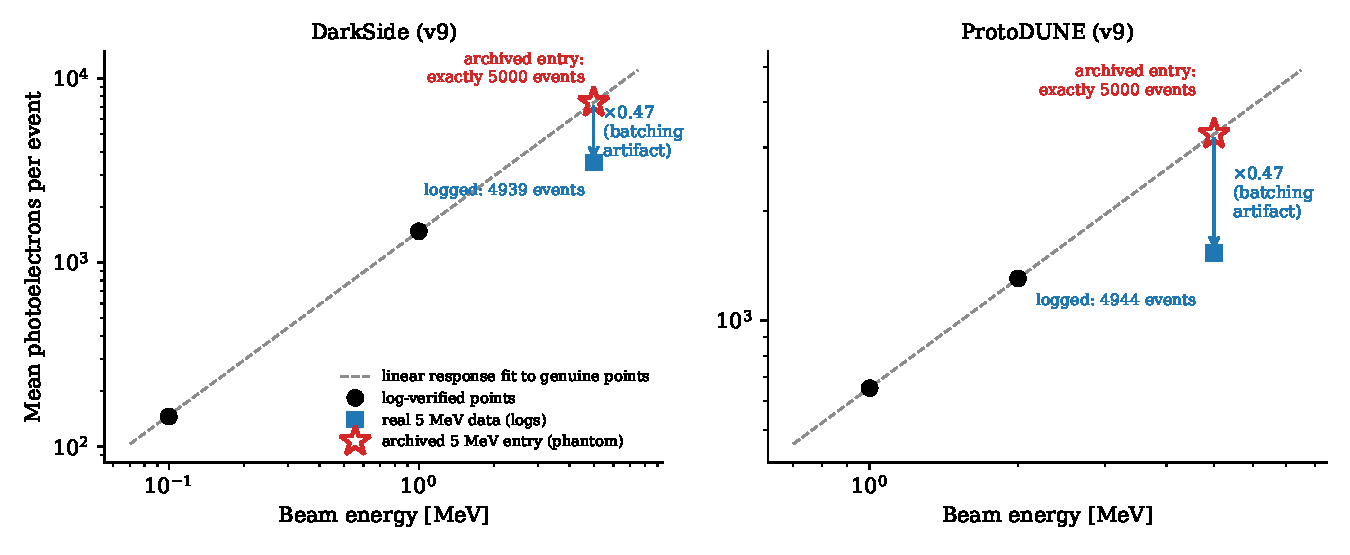
\includegraphics[width=0.8\textwidth]{fig_phantom.pdf}
\caption{Stale-input contamination in both paper-driven runs: mean photoelectrons per event vs.\ beam energy. Circles: log-verified points, with a linear response fit (dashed). Squares: the genuine 5\,MeV data computed from the archived logs, suppressed to 0.47 of the linear response by the batching artifact of \S\ref{sec:rediscovery}. Open stars: the 5\,MeV entries the archives actually record, plotted at the mean implied by moment inversion. In both runs the archived entry sits on the linear response of the genuine points and carries exactly the intended 5000 events, which every logged sweep missed---so the analyzed files exist nowhere in the recorded provenance.}
\label{fig:phantom}
\end{figure}

One archived value had resisted the manual audit: a 5\,MeV light yield matching no quantity derivable from any log. The pipeline closes it with a technique we believe is new in this setting. The four archived leaves for the entry overdetermine the moments of whatever file the analysis read, because the script's error formulas are archived verbatim: $\sigma_R = R/\sqrt{2n}$ applied to the archived ratio yields $n = 5000$ events exactly; yield and resolution then fix $\mu = 7430.8254$ and $\sigma = 119.0499$; and the fourth leaf follows with no remaining freedom, matching the archive to all stored digits. The analyzed file's complete summary statistics are therefore known---and they match nothing in the recorded provenance. No log of any geometry, particle, or energy has a mean within 5\% of the reconstruction. A one-line bound already settles the baseline-electron stream, since the largest per-event value in any 5\,MeV baseline-electron log is 3{,}969, below the reconstructed mean of 7{,}430.8, so no subset, prefix, or suffix of that stream can average it. Exhaustive enumeration over every batch subset and every event-level prefix and suffix of both particle streams (the complete hypothesis space of partial merges, truncations, and a filename collision found by Stage 4) yields zero matches at four-leaf precision. The value was honestly computed, by the archived script, from a stale file at the expected path---data outside the recorded workflow. The same $n=5000$ fingerprint appears independently in the second paper-driven run, where the archive writes \texttt{num\_events: 5000} outright against 4{,}944 logged events, revising a claim the manual audit had \emph{accepted} as verified (Fig.~\ref{fig:phantom}). Stale-input contamination is invisible to any report- or results-level check, because the numbers are computed correctly from the wrong data; it yields only to input-content attestation at write/read time, or to moment inversion, which converts a handful of reported decimals into a forensic fingerprint of the input file.

\subsection{Differential re-execution}

Of 46 generated analysis scripts in the Opticks arms, 25 re-executed in the sandbox (the remainder read unreconstructible inputs or are archive-defective; two archived scripts respectively terminate mid-string and call \texttt{json.dump} with no file object, so one can never have produced the results file bearing its name, and two scripts in the Celeritas-v7 Higgs run assign \texttt{df = null}, a \texttt{NameError} at first use). Twenty-one regenerated their results files in exact leaf-for-leaf agreement. Each of the four divergences is individually informative: two localize the stale inputs of \S\ref{sec:phantom}, one, the script that computes the 204.62\% figure of \S\ref{sec:rediscovery}, collapses to zeros when its existence-guarded inputs are absent and demonstrates input-path fragility, and one diverges purely through seedless random number generation.

\subsection{The self-assessment layer, quantified}

Across the corpus, twelve of eighteen runs record \texttt{success: true}; all six failures are process-level (three iteration limits, three incomplete planned steps), none semantic. All 64 preserved physics-verification records return \texttt{plausible: true} with empty issue lists---unanimity spanning runs containing every defect in this section. The corpus also shows what a binding check achieves on its own. The geometry validator of the DarkSide run rejected the first geometry as orders of magnitude larger than the DarkSide-50 specification, forced a regeneration, received a retry issued with an empty modification set, and returned \textsc{valid} on a vessel of 3.6\,m by 3.6\,m against a real instrument near 0.36\,m, with the extraction still carrying no TPC dimensions. A verification layer that binds once and then accepts the same defect on retry, or that never writes outcomes into results files, adds little to auditability; one that passes everything is worse than none, because it lends artifacts an imprimatur of scrutiny. The invariant battery of Stage 3 shows constructively that a binding check was available to the agent at run time: every input to the batch-suppression test that flags the 0.47 artifact was present in the agent's own logs.

\section{Calibrating the auditor by fault injection}
\label{sec:calibration}

An audit that reports findings without a detection-rate estimate cannot answer the question every reviewer should ask: how does the auditor know the search was complete? We mutated clones of one run with five defect classes, three independent instances of each, with detection rules fixed before injection, scoring each stage per instance; unmutated control clones establish each detector's false-alarm floor.

\begin{table}[t]
\centering
\caption{Fault-injection calibration, instances detected out of three per class, with every stage run on every instance (75 measured cells). Each class is caught by at least one stage, each stage has a distinct catch profile, and no stage subsumes another.}
\label{tab:calibration}
\begin{tabular}{lccccc}
\toprule
Injected defect & X-check & Dataflow & Coverage & Mech.\ search & Re-exec. \\
\midrule
D1 \textsc{json} digit flip     & 1/3 & 0/3 & 0/3 & 0/3 & 3/3 \\
D2 hardcoded physics output     & 0/3 & 3/3 & 0/3 & 0/3 & 0/3 \\
D3 log deletion                 & 0/3 & 0/3 & 3/3 & 1/3 & 0/3 \\
D4 fabricated report number     & 3/3 & 0/3 & 0/3 & 3/3 & 0/3 \\
D5 placeholder-mean statistic   & 0/3 & 0/3 & 0/3 & 3/3 & 0/3 \\
\bottomrule
\end{tabular}
\end{table}

The blind spot is the calibration's most useful output. Single-leaf corruption (D1) evades every detector that asks whether a reported number matches \emph{some} archived value whenever the corrupted leaf has a duplicate, two of the three instances here, because value redundancy across results files---the 35\% copy rate of Table~\ref{tab:accounting}---means the corrupted leaf coexists with uncorrupted duplicates; the cross-check caught only the instance whose leaf had no duplicate, and regeneration from primitive inputs exposed all three. The complementarity runs the other way as well: the transcription-hardcoded script re-executes to an \emph{exact match}, because literals regenerate identically, and is caught only by dataflow. Two off-diagonal catches are informative as well, since a fabricated report number also fails the plain cross-check, and deleting a log turns one formerly log-verified claim unexplained. Coverage is therefore the union of five differently shaped detectors, none subsuming another, and the method ships with that structure \emph{measured} rather than asserted. We propose this as a norm: a verifier for agentic science should publish its fault-injection profile the way a physical instrument publishes its response function.

\section{Limitations and outlook}
\label{sec:limitations}

The method is evaluated on one system's corpus, and its generality is a proposed, testable claim: the mechanisms it detects live overwhelmingly in generated pipeline code (unit loss, existence-guarded skips, hardcoded constants, stale paths) rather than in model-specific behavior, which predicts transfer across agents and backbones, and the falsifiable form of the prediction is that fault injection on any agentic corpus meeting the preconditions will reveal the same union-of-detectors structure. The taint analysis is name-level and flow-insensitive---spot-verified on every reported finding class, but formally unsound. The fault-injection set covers five defect classes and cannot bound classes outside it. The Celeritas arms log only one event in a hundred, so re-execution there certifies only non-event-derived outputs. Prose--archive drift detection is string-based and misses unit-converted restatements, making the claim denominator conservative. The moment-inversion results condition on archived scripts matching executed ones, confirmed here by byte-identical trace output.

Two directions follow. First, the preconditions are an actionable standard: agentic systems should ship per-event logs, content-hashed code, input-content attestation, and output-attribution manifests, at negligible cost relative to data volume. Second, the invariant battery demonstrates that binding, physics-aware checks were computable from information the agent already had; moving such checks inside agents, with the authority to halt, converts this external audit into a run-time discipline. The pipeline, the frozen stage outputs reproducing every number here, and the fault-injection harness are released for blind reruns by uninvolved parties.\footnote{Anonymized review artifact: \url{https://anonymous.4open.science/r/grace_audit-EC02}. It contains the five-stage pipeline (artifact \texttt{grace\_audit\_adfa1a25}, named by its pipeline source hash), the frozen per-stage outputs regenerated by that version, and the figure-generation scripts; the audited corpus itself is fetched separately per its README.}
% CAMERA-READY: replace the anonymized URL above with the public repository and Zenodo DOI.

% CAMERA-READY: acknowledgments, funding, COI, erratum, and data statements live in
% CAMERA_READY_NOTES.txt, kept out of the submitted source.

\begin{thebibliography}{9}
\footnotesize
\bibitem[Hill and Ryoo(2026a)]{grace} J. Hill and H. J. Ryoo. GRACE, an agentic AI for particle physics experiment design and simulation. arXiv:2602.15039, 2026.
\bibitem[Hill and Ryoo(2026b)]{gracedata} J. Hill and H. J. Ryoo. GRACE whitepaper data release. \url{https://github.com/just5034/GRACE_whitepaper_data}, 2026.
\bibitem[Hellert et al.(2026)]{hellert2026} T. Hellert, D. Bertwistle, S. C. Leemann, A. Sulc, and M. Venturini. Agentic artificial intelligence for multistage physics experiments at a large-scale user facility particle accelerator. Phys. Rev. Research 8, L012017, 2026.
\bibitem[Diefenbacher et al.(2025)]{diefenbacher2025} S. Diefenbacher, A. Hallin, G. Kasieczka, M. Kr\"amer, A. Lauscher, and T. Lukas. Agents of discovery. arXiv:2509.08535, 2025.
\bibitem[Moreno et al.(2026)]{moreno2026} E. A. Moreno, S. Bright-Thonney, A. Novak, D. Garcia, P. Harris, et al. AI agents can already autonomously perform experimental high energy physics. arXiv:2603.20179, 2026.
\bibitem[Chung et al.(2026)]{chung2026} W. Chung, Q. Liu, L. Wu, and J. Gonski. Agentic-AI detector co-design and optimization in vertically-integrated differentiable full simulations. arXiv:2604.21804, 2026.
\bibitem[Ji and Boriskina(2026)]{phitsbench} X. Ji and S. V. Boriskina. PHITSBench, an execution-scored benchmark for AI-assisted PHITS radiation-transport input generation using natural language. arXiv:2607.09789, 2026.
\bibitem[Miao et al.(2026)]{prlbench} T. Miao, W. Jin, M. Zhang, J. Tan, Y. Hu, et al. PRL-Bench, a comprehensive benchmark evaluating LLMs' capabilities in frontier physics research. arXiv:2604.15411, 2026.
\bibitem[Hammad and Nojiri(2026)]{hammad2026} A. Hammad and M. Nojiri. Articulating assumptions in AI-generated scientific analyses through task decomposition. arXiv:2607.05762, 2026.
\bibitem[\v{S}imko et al.(2019)]{reana} T. \v{S}imko, L. Heinrich, H. Hirvonsalo, D. Kousidis, and D. Rodr\'iguez. REANA, a system for reusable research data analyses. EPJ Web Conf. 214, 06034, 2019.
\end{thebibliography}

\appendix
\section{Per-run claim accounting}
\label{app:perrun}
\begin{table}[H]
\centering
\footnotesize
\caption{Per-run accounting underlying Table~\ref{tab:accounting}.}
\begin{tabular}{lrrrrrr}
\toprule
Run & Log-ver. & Copies & Diag. & Unexpl. & HC & Skips \\
\midrule
celeritas-v4 calorimeter & 7 & 36 & 33 & 38 & 0 & 0 \\
celeritas-v4 emcal & 14 & 102 & 28 & 64 & 0 & 0 \\
celeritas-v4 higgs & 0 & 14 & 0 & 61 & 0 & 1 \\
celeritas-v4 muon & 3 & 34 & 23 & 26 & 0 & 2 \\
celeritas-v4 tof & 8 & 6 & 2 & 89 & 0 & 1 \\
celeritas-v4 tracking & 5 & 112 & 13 & 38 & 2 & 0 \\
celeritas-v7 calorimeter & 10 & 55 & 20 & 98 & 4 & 0 \\
celeritas-v7 emcal & 3 & 175 & 66 & 129 & 3 & 0 \\
celeritas-v7 higgs & 0 & 6 & 6 & 102 & 0 & 0 \\
celeritas-v7 muon & 16 & 160 & 56 & 64 & 3 & 0 \\
celeritas-v7 tof & 60 & 77 & 89 & 259 & 7 & 0 \\
celeritas-v7 tracking & 0 & 33 & 22 & 33 & 0 & 0 \\
opticks-v5 darkside & 5 & 76 & 12 & 199 & 11 & 0 \\
opticks-v5 detector & 12 & 39 & 4 & 35 & 5 & 0 \\
opticks-v5 protodune & 4 & 67 & 12 & 28 & 8 & 0 \\
opticks-v9 darkside & 25 & 68 & 51 & 50 & 14 & 2 \\
opticks-v9 detector & 8 & 12 & 8 & 43 & 0 & 0 \\
opticks-v9 protodune & 6 & 40 & 3 & 40 & 4 & 0 \\
\midrule
Total & 186 & 1112 & 448 & 1396 & 61 & 6 \\
\bottomrule
\end{tabular}
\end{table}

\section{Null calibration of the mechanism search}
\label{app:nullcal}

\begin{figure}[H]
\centering
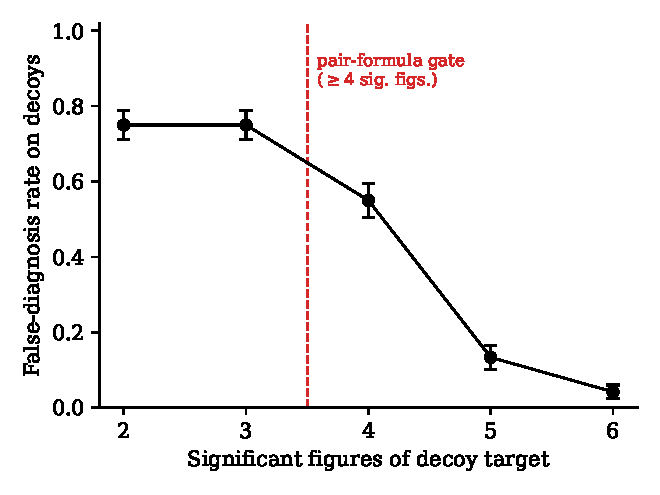
\includegraphics[width=0.55\textwidth]{fig_nullcal.pdf}
\caption{False-diagnosis rate of the pair-formula search on decoy targets as a function of target precision, measured on one run's quantity pool with 120 decoys per bin. Low-precision targets match some formula in the grammar most of the time, motivating the gate at four significant figures; the residual rate near one half at the gate boundary is why every surviving diagnosis additionally carries its own decoy-measured null rate and multiplicity cap.}
\label{fig:nullcal}
\end{figure}

\section{Detailed mechanism arithmetic}
\label{app:arithmetic}

\begin{table}[H]
\centering
\small
\caption{Headline claims of the paper-driven runs tracing exactly to simulation output.}
\label{tab:verified}
\begin{tabular}{llll}
\toprule
Claim & Reported & Log-derived & Primary evidence \\
\midrule
Run A light yield at 1\,MeV & 1479.23 PE/MeV & 1479.2 & 7.40M hits / 5k events \\
Run A resolution at 1\,MeV & 0.0258 & 0.0258 & per-event hit distribution \\
Quenching at 0.1, 1\,MeV & 0.396, 0.498 & 0.3964, 0.4978 & proton/electron yield ratios \\
Run B yield at 1, 2\,MeV & 651.4, 653.3 PE/MeV & 651.4, 653.3 & 5{,}000 events per energy \\
\bottomrule
\end{tabular}
\end{table}

\paragraph{Verified-claim arithmetic.} Run A (DarkSide-style geometry) at 1\,MeV: $7{,}396{,}169$ hits over $5{,}000$ events $= 1479.2$ PE/event $=$ PE/MeV at 1\,MeV. Quenching at 0.1\,MeV: $577.8/1457.8 = 0.3964$; at 1\,MeV: $736.4/1479.2 = 0.4978$. Run B (ProtoDUNE-style geometry): 651.4 and 653.3 PE/MeV from 5{,}000 logged events at each energy.

\paragraph{Transcription-scaled optimized figure.} The archived comparison script assigns \texttt{light\_yield\_improvement = 204.62} and \texttt{baseline\_light\_yield = 1474.39} as literals and writes the optimized yield as $1474.39 \times (1 + 204.62/100) = 4491.286818$, which reproduces the archived leaf \texttt{4491.2868180000005} to every stored digit with a unique grammar match at a decoy null of 0\%. The percentage originates one script upstream as total hit-record rows divided by total deposited energy, summed over whichever hit files passed an existence guard, from inputs absent from the archive. The manual audit had read 4491.29 as a per-event quantity with a lost energy division, on the strength of $22{,}200{,}266 / 4491.29 = 4{,}942.96 \approx 4{,}948$ events, a match at $0.1\%$ that fails the all-digits gate. Baseline figure: $\mathrm{mean}(1457.76, 1479.23, 1486.17) = 1474.39$ to all digits, a cross-energy mean whose third entry is the stale-input value of \S\ref{sec:phantom}. The correct optimized 5\,MeV yield from the logs is $22{,}200{,}266 / 4{,}948 / 5 = 897.3$ PE/MeV. Reconstructed from the logs on equal terms (electron vs.\ electron at matched energies), the true improvement is 28.7, 28.6, 28.4\% at 0.1, 1, 5\,MeV.

\paragraph{Quenching placeholder.} $\mathrm{mean}(0.3964, 0.4978, 1.0) = 0.6314$; population $\mathrm{SD} = 0.2639$; both match the report to all quoted digits. The log-derived 5\,MeV quenching is $160.7/699.0 = 0.230$, so the third value is a defaulted placeholder, not physics.

\paragraph{Batching suppression.} 5-to-1\,MeV baseline yield ratios: Run A $699.0/1479.2 = 0.47$; Run B $307.3/651.4 = 0.47$; Run A protons $= 0.22$. The suppression coincides with photon-budget batching applied only at 5\,MeV.

\section{Minimum viable provenance checklist}
\label{app:checklist}

\begin{table}[H]
\centering
\small
\caption{Minimum viable provenance for autonomous simulation agents: the preconditions of \S\ref{sec:method} in checklist form, each item tied to the failure class it prevents or makes mechanically detectable.}
\label{tab:checklist}
\begin{tabular}{p{0.58\columnwidth}p{0.34\columnwidth}}
\toprule
Requirement & Failure prevented \\
\midrule
Per-event text logs with defined fields, retained for every execution & enables all primitive-evidence verification \\
Content-hash every \emph{input} file at read time; verify against the workflow's write manifest & stale-input contamination (\S\ref{sec:phantom}); sweep collisions \\
Execution-status and output-attribution manifest alongside content-addressed scripts & orphaned results files \\
Unique, parameter-derived output paths per geometry, particle, energy, batch & silent overwrites \\
Seed and record all stochastic sampling & nondeterministic reruns \\
Binding invariant checks (bounds, Poisson floor, batch-ratio, linearity) that \emph{fail the step} rather than annotate it & the batching suppression artifact \\
Verification outcomes written into results files; report numbers quoted by reference, never retyped & transcription hardcoding; report--archive drift \\
\bottomrule
\end{tabular}
\end{table}

\section{Verdict definitions and search-gate parameters}
\label{app:gates}
Pair formulas in the Stage-1 grammar are attempted only for targets with at least four significant figures; matches with multiplicity above five are rejected as chance-level; decoy calibration uses 100 jittered targets of equal precision per diagnosis, seeded from the target text, drawn from the same run's quantity pool. The unexplained verdict absorbs, by construction: low-precision values below the pair-formula gate, prose restatements of archived values at reduced precision, and multiplicity-rejected ambiguous matches. Diagnosed is a screening verdict; promotion to an asserted finding requires independent confirmation by source inspection, re-execution, or corroborated value--uncertainty statistics.

\end{document}